% Co-authored-by: cherusk <10729954+cherusk@users.noreply.github.com>
\documentclass[11pt,a4paper]{article}
\usepackage[utf8]{inputenc}
\usepackage[T1]{fontenc}
\usepackage{libertine}
\usepackage[libertine]{newtxmath}
\usepackage{amsmath}
\usepackage{graphicx}
\usepackage{xcolor}
\usepackage{booktabs}
\usepackage{subcaption}
\usepackage{titlesec}
\usepackage{parskip}
\usepackage{hyperref}
\hypersetup{hidelinks}
\usepackage[margin=2.6cm]{geometry}

% Draft-v2 (holder's word 2026-11-21: the data is authoritative): all
% four figures regenerate from the evidence bundles by make_figures.py
% (the regen contract); the tables carry the regenerated series. The
% bend prints as the NARROW kind (receipt corrected on the data); the
% transfer widening prints at the change minute. Registry identities
% never print; they resolve at the evidence port.

\title{The Connectome --- A Living Empirical Causal Model of\\ Changing Substrates}
\author{
  Matthias Tafelmeier \\
  Independent Scientist \\
  Hof, Germany \\
  \href{https://orcid.org/0009-0005-7399-5584}{ORCID: 0009-0005-7399-5584}
}
\date{}

\begin{document}
\maketitle

\begin{abstract}
Autonomous agents that tend a shared substrate can measure it while it
runs: couplings are discovered by probing, response curves carry error
bars, and the curves compose across hops. The result is a
\emph{connectome} --- an empirical causal model of a live world, every
number in it measured, never assumed. The predecessor papers built it
and steered through it. This paper turns to the model itself and asks
the question their line of work ends at: what kind of thing is such a
model when the substrate will not hold still? The answer is that it has
a life, and that the whole life is measurable in the model's own units.
It is \emph{born} at a real cost of probing. It \emph{decays} as the
world changes --- measurably, and differently per kind of change --- and
it \emph{notices}: its own uncertainty bars are the alarm, with no
external monitor. It \emph{heals} at a price, the repair aimed where
the bars broke. It \emph{endures} load, with the walls named as walls.
It \emph{carries} into a new regime, the widening of its survey fitted
to the blast radius of the change. And its knowledge is \emph{priced}:
held at fresh level through a busy evening of scheduled and unscheduled
change, at a cost that fell unevenly across the tending group ---
cheaper than an un-updated map's calm ignorance where it is cheaper, and
honestly not where it is not. One claim, carried by receipts from a
live measurement campaign; every boundary printed as a boundary.
\end{abstract}

\noindent\textbf{Keywords:} autonomous agents, multi-agent systems,
connectome, causal model, model lifecycle, model decay, model
maintenance, uncertainty, self-adaptive systems, live systems

\section{Introduction}
\label{sec:intro}

When autonomous agents tend the same substrate, each one's parameter
changes travel through the substrate into the others' readings. The
prior work of this lineage established that this hidden coupling is
measurable without central observers and without stopping the system:
edges are discovered by guardrail-bounded probing between the agents
themselves~\cite{p1}, each edge yields a response curve with per-point
error bars~\cite{p2}, and the measured curves compose across nonlinear
hops and converging paths~\cite{p3}. The last paper asked what such a
model can \emph{do}, and answered it: a promise can be steered through
the composed model, refused when the measured range says no, kept
through drift, and priced in rounds and waterings~\cite{p4}.

This paper asks the question that line ends at. The model those papers
built --- the substrate's \emph{connectome} --- is not a file. On a
live substrate it is an object with state, and the state can go wrong.
What kind of thing is it, such that it can age? And is the aging
itself measurable --- not just the model working or failing, but the
whole life of the model, stage by stage, in its own units?

The claim, in one sentence, carried by the campaign this paper
receipts: \emph{a measured model of a changing substrate has a whole
life --- it is born at a cost, decays measurably as the world changes,
notices its own staleness, heals at a price, endures load, and carries
into new regimes --- and every stage of that life is measurable; and
its knowledge is priced: cheaper than guessing, luck, or hindsight
where it is cheaper, and honestly not where it is not.}

The stages, in the order the campaign receipts them:

\begin{enumerate}
\item \textbf{Birth.} Building the model costs real, honest units: a
full response ladder prices one relationship to the fixed bar in
amortized running time, the measuring turn rotating among the members
(\S\ref{sec:birth}).
\item \textbf{Decay, and noticing.} The model goes stale per
\emph{kind} of change --- a readout slides, an influence doubles, a
response bends, a direction flips --- and all four kinds break its
uncertainty structure locally, each with its own breadth, magnitude,
and timing; the alarm is the model's own worst bar
(\S\ref{sec:decay}).
\item \textbf{Healing.} Repair works and costs, per kind: the re-walk
is aimed where the bars broke, and its price reads in the members' own
trials (\S\ref{sec:healing}).
\item \textbf{Endurance.} Keeping is priced over time and under load;
the walls --- turn-taking throughput, peers in motion --- are measured
and named as walls (\S\ref{sec:endure}).
\item \textbf{Carry.} A model built under one regime served under
another, whole-regime change; the survey widened to fit the blast
radius, the protocol unchanged (\S\ref{sec:carry}).
\item \textbf{The price.} One busy evening: three scheduled changes
and one unscheduled push, seventeen minutes, the knowledge held at
fresh level, the cost distributed unevenly across the group, and every
price read absolutely between what a never-updated model buys (calm
ignorance) and what unlimited hindsight would buy
(\S\ref{sec:price}).
\end{enumerate}

One containment rules everything below, as in the predecessor. The
comparison is contained: no external model family appears. The honesty
of every price is carried by anchors computed from the same runs ---
a never-updated model (do nothing: keep the build-time bars while the world
moves), a random arm (declared analytically from the bench's dial
geometry), and an oracle (unlimited hindsight, computed after the fact
from the recorded truth). Every number in this paper reads absolutely
between those anchors or is declared as owed.

\emph{What flew is the smallest set of runs that exercises the whole
life.} The reference group on a quiet bench, the four change kinds of
the bench's event grammar, one multi-change evening, and one regime
change --- a proof of concept, deliberately small, in the lineage's
standing tradition: the smallest complete object on which each claim
can be checked against total truth. Scaling is the open direction the
boundaries point at (\S\ref{sec:boundaries}), and the closing
boundary is named outright: everything here is measured where truth
was known. The open era is models of substrates where it is not.

\section{The substrate and the connectome}
\label{sec:orientation}

\emph{Substrate.} The substrate is whatever the agents tend:
physical, computational, or mathematical. In this campaign it is a
live bench of coupled nodes; each node exposes parameters (dials) and
readings (objectives), and a change of one node's dial travels
through the planted couplings into other nodes' readings. A truth
channel records what was actually planted at every tick --- the
answer key. It is never read at decision time; it scores after the
fact.

\emph{The pieces, told plainly.} Guardrail-bounded probing between
the agents discovers the hidden couplings --- the \emph{edges},
measured without stopping the system~\cite{p1}. Each edge yields a
response curve with per-point error bars, honest against the
substrate's noise~\cite{p2}. And the curves \emph{compose}: chained
across hops, they predict far-end response~\cite{p3}.

\emph{The connectome, and its one function.} Measured edges, curves,
and their composability together are the substrate's
\emph{connectome}: an empirical causal model --- every number in it
measured against the world or retired on measured evidence, never
assumed. The connectome \emph{maps}: its measured structure --- edges,
weights, bases, bars --- is a picture of the substrate's territory.
The connectome also \emph{predicts}: planning through it, refusing
when a bar is too wide, correcting by predicted effect. The
predecessor paper called this picture simply \emph{the
map}~\cite{p4}; wherever the word map appears below, it keeps that
sense --- the mapping, one function of the model --- while the thing
with a life is the connectome itself
(Figures~\ref{fig:connectome} and~\ref{fig:curves}).

\emph{Tenders, named once.} Everything the model does, somebody does:
the members that tend the substrate --- probing it, watching the
readings against the curves, re-walking what broke --- are
\emph{tenders}. They tend; they never optimize. Their keeping
grammar, and the wishes a holder may declare through the map, are the
predecessor's subject~\cite{p4}; this paper takes the tenders as
given --- the model's hands --- and claims nothing new about them.

\begin{figure}[!ht]
\centering
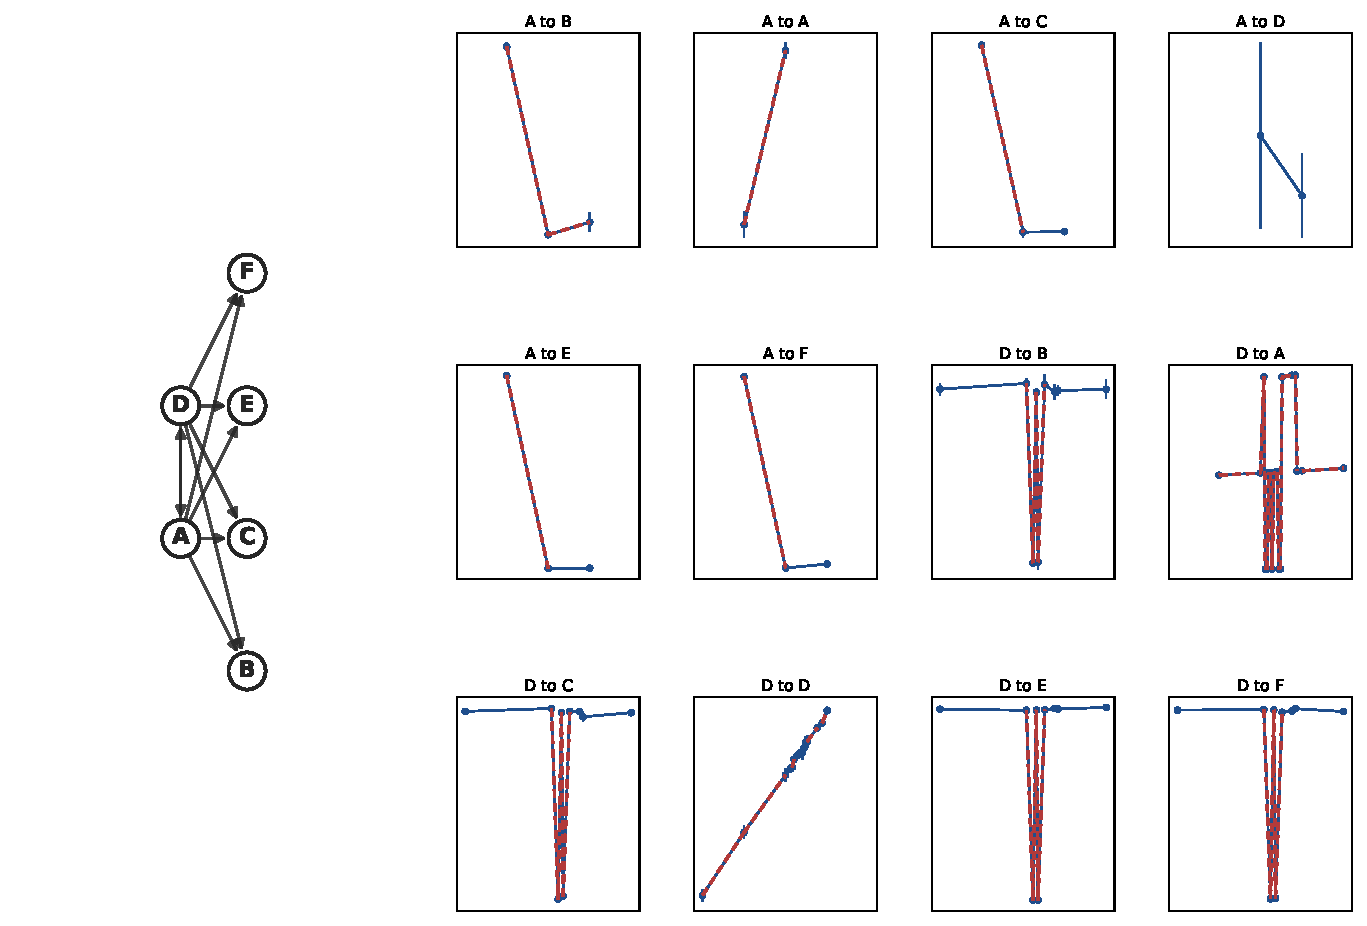
\includegraphics[width=\linewidth]{figures/connectome}
\caption{The connectome: the whole measured map of one live system.
All six members and all twelve measured couplings of one snapshot ---
thick blue arrows walked in full, thin gray arrows whose walk had
just begun; a member's reading of itself loops at its node. Every
coupling's own curve follows on the next page.}
\label{fig:connectome}
\end{figure}

\begin{figure}[p]
\centering
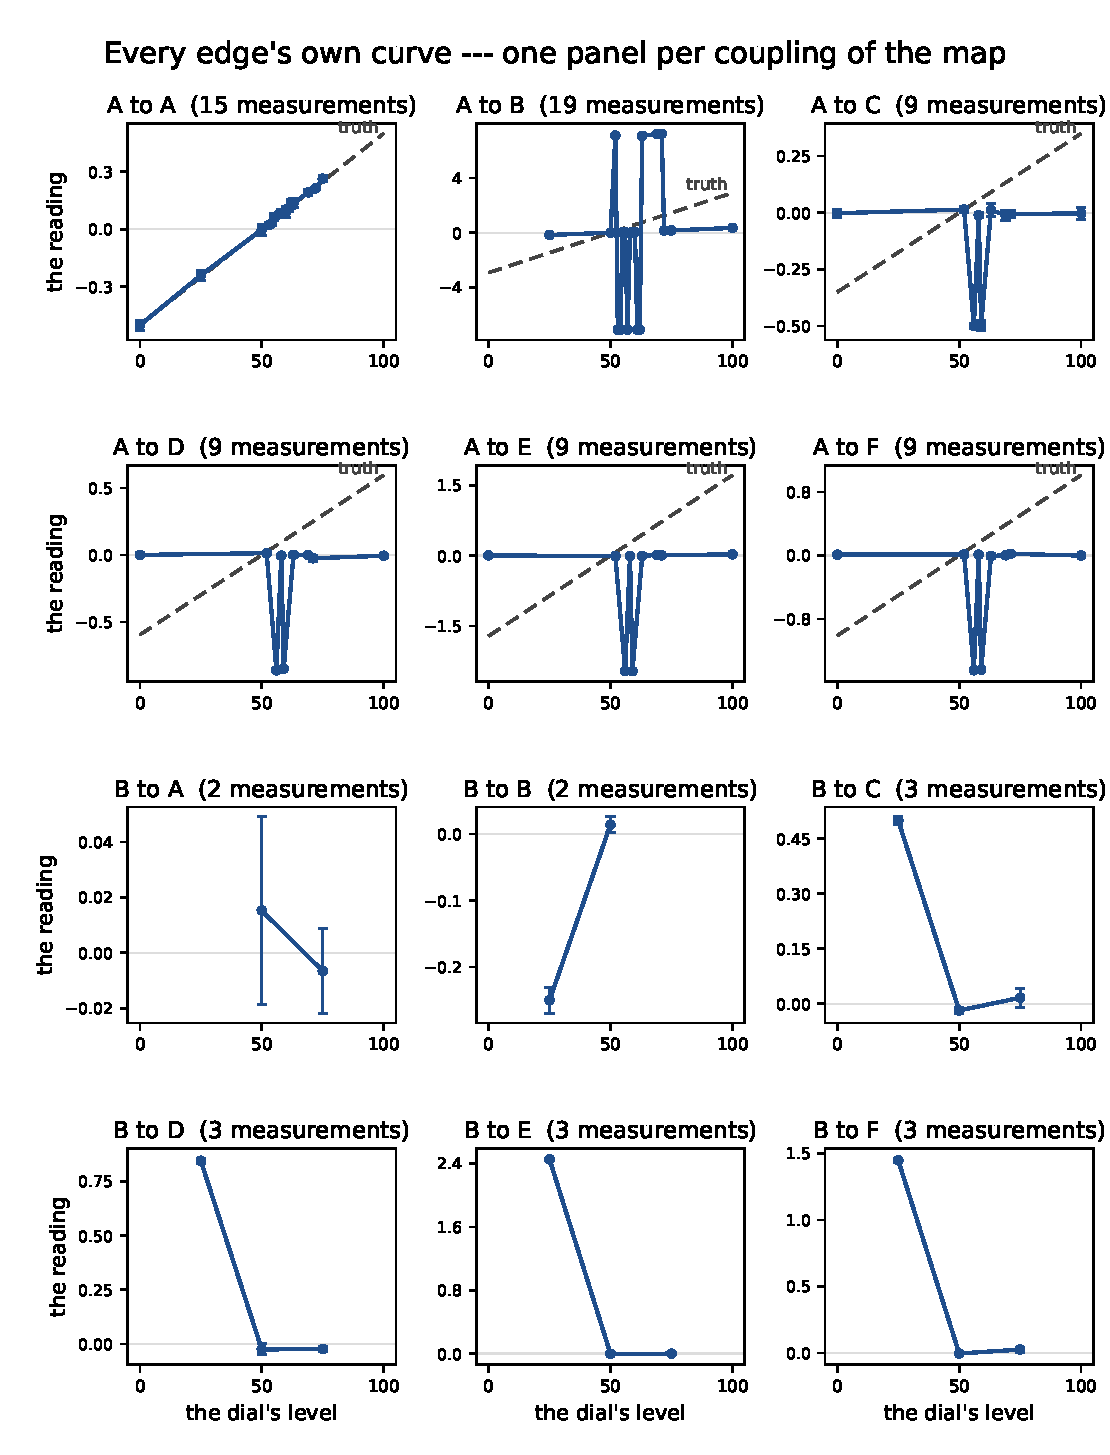
\includegraphics[width=\linewidth]{figures/curves}
\caption{Every edge's own curve --- one panel per coupling of the map
in Figure~\ref{fig:connectome}, titled by its pair. Each dot is one
probe's record: the receiver's median reading while the sender's dial
was held at that level minus its median at the resting position
(dial 50) --- the change from rest, with its honest uncertainty as the
capped line (often smaller than the dot: the instrument is precise).
The line joins consecutive records from low to high dial level. The
dashed line is the scenario's true response for that edge, computed
from its declared coupling structure with every other member at rest
and likewise measured from the resting position. The self-reading's
records lie on their truth line to the digit; the cross-edges'
records do not follow their true responses --- an open instrument
question for live rooms, where the receiving members' own dials may
move during a probe. The late prober's node is not yet identified, so
its panels carry no truth line. The count in each title is the number
of records so far.}
\label{fig:curves}
\end{figure}

\emph{What kind of object, that it can age.} The connectome is a
\emph{store with state}, not a file of curves: measured levels per
dial, live brackets, per-gap pricing, retired (converged) parameters,
and error bars that are themselves claims about the world. A curve
does not rot; a stored claim about a living substrate does --- and it
is the state that decays. It is \emph{partial} by design: measured
where knowing was worth the trials, deliberately holed where it was
not; the holes are honest admissions of not knowing, never filled by guesswork. It is
\emph{persisted}: the model outlives the walkers that built it, which
is precisely why it can age. It is \emph{served}, not just held:
consumed live through its doors by planning, by the watch, by the
re-walk. And its decay is \emph{local}: when the world moves, the
error concentrates where the structure changed --- the model's own
error is the compass that aims its repair. Birth, decay, notice,
heal, endure, carry: every stage that follows is a measurement on
this object.

\emph{Causal, in the interventional sense.} The connectome is a
causal model on three constitutive ingredients. \emph{Variables}: the
dials and the readings. \emph{Directed structure}: the curves are
measured by asymmetric intervention --- one side moves, the other
answers --- so where the measurement finds nothing, the arrow is absent and a sign flip is
tracked as the world's own change. \emph{Interventional semantics}:
the model is built by doing, answers questions of doing, refuses when
its bars say uncertain, and every arrow carries its uncertainty. What
is deliberately \emph{not} claimed --- counterfactual queries and
identification theory --- is printed as a boundary, with the named
outlook, in \S\ref{sec:boundaries}.

\section{The instrument: what makes a life countable}
\label{sec:instrument}

Every claim in this paper rests on measurements of the model's own
state, so the rules that make those measurements countable are part
of the instrument.

\emph{The unit is the bar.} The model's honesty unit is the
uncertainty bar on a curve. Every run of this campaign fixed its bar
at the same value ($0.02$) and cites the fixed value in every
receipt; knowledge, decay, healing, and price all read in this unit.
No verdict is ever taken from a run's badge or summary.

\emph{Everything is recorded.} Every run writes the same diary ---
per tick and per event --- and the truth channel records what was
actually planted throughout. Nothing planted is visible to the
members; the truth exists only to score. All numbers in this paper
are recomputed from these recordings.

\emph{Change is declared.} The bench carries an event grammar: each
change is an event with a destination and a declared clock --- wall
seconds or ticks, named per run --- and the drift schedule is part
of the scenario, never a surprise to the record (it is always a
surprise to the model, which never reads it). Where a warm run
compressed a tick-denominated event into the model's first minutes,
the compression is printed with the run, not hidden.

\emph{No silent defaults.} Every number is computed from the run's
own measurements or from a declared term; where a precise table is
not yet computed (the per-trial economics, the random arm's exact
constant), the debt is declared in the text, never papered over.

\emph{Honest close.} A run that misbehaves is a receipt: the
anomaly is recorded, the flaw fixed, and the experiment re-flown. Three
experiments of this campaign exercised that rule; the re-flown numbers are
the ones printed here.

\section{Birth: what building costs}
\label{sec:birth}

The model is born by walking. A dial is swept level by level across
its range --- a full ladder --- and the receiver's answers, with their
bars, become the curve; the edge is done when the bar is met. The
birth receipt: a ladder of a hundred and one levels at the fixed bar
amortizes to between one and one-and-a-half levels per minute of run
time, with the measuring turn rotating among the members so that no
one walker monopolizes the substrate --- the same turn-taking discipline
that reappears under load (\S\ref{sec:endure}) and under regime
change (\S\ref{sec:carry}).

Build spans and walking cadence were measured across the reference
grid, per group size and coupling, in the campaign that also produced
the load walls of \S\ref{sec:endure}; the curve-level economics
themselves are the predecessor's published result~\cite{p2} and are
cited, not re-run. What is new here is the \emph{amortized run
price} of a whole relationship --- the number a keeper must budget
before the first promise is ever declared: the model's birth is not
free, and its cost is a receipt, not an estimate.

\section{Decay, and noticing}
\label{sec:decay}

The world changed in four named ways, one kind per run, each event
exact in the truth record --- destination, clock, travel --- and each
run asked the same question: what does this kind of change do to the
model's uncertainty structure? Table~\ref{tab:kinds} gathers the
four answers.

\begin{table}[!ht]
\centering
\small
\begin{tabular}{@{}p{0.22\linewidth}p{0.28\linewidth}p{0.40\linewidth}@{}}
\toprule
\textbf{Change kind} & \textbf{What changed in the world} &
\textbf{The model's response (uncertainty bars; fixed bar 0.02)} \\
\midrule
the sensor slides (readout drift) & every reading on one node slowly
lies & promise breaks; detected; re-walked at a cost of $\sim$200
extra trials ($\sim$$+50\%$) \\
a relationship doubles (weight $1{\to}2$) & one influence's strength
doubles & LOUD: one relationship's uncertainty $\sim$0.77 for the
whole window (born into the event); one neighbor stirred (0.31); ten
calm \\
a response bends (linear$\to$saturation) & one node's curve changes
shape & NARROW: at the exact bend, two gap-bars jump ($0.03 \to 0.54$,
${\sim}27\times$ the bar) and hold to the close; the rest of the curve
stays low; two stretches tighten \\
a relationship reverses ($+0.7{\to}{-}0.7$) & one influence flips
direction & LOUDEST: epicenter $0.02 \to 1.12$ ($56\times$ the bar);
sisters calm; detected and re-measured \\
\bottomrule
\end{tabular}
\caption{The four kinds of change and what each did to the model.
Public words throughout: the world moved on purpose, the model's
bars answer. Reading line: all four kinds announce themselves ---
three with broad breaks of distinct magnitude, the shape-bend with a
narrow spike exactly where the curve bent; in this run the bend's
heal was starved and its flag stood to the close (the named
follow-up, \S\ref{sec:boundaries}).}
\label{tab:kinds}
\end{table}

\emph{The slide.} Every reading on one node began to lie, at a
declared rate from a declared cue, capped. The model had no external
monitor --- and needed none: readings landed outside what the curves
promised, the stale prediction breaking \emph{is} the detection, and
the re-walk began. The predecessor published this arc's mechanism
with stable numbers~\cite{p4}; this campaign's contribution is the
heal-cost signature in the members' own trials
(\S\ref{sec:healing}).

\emph{The climb.} One influence's weight doubled, and the event's
tick cue compressed into the model's own birth: the map was still
building when the world it was mapping changed underneath it. The
result is the section's quietest finding: the break was localized
anyway. One relationship --- the changed one --- carried bars around
$0.77$ for the entire window, roughly ten times its sisters; one
neighbor stirred at about a third; ten curves stayed calm at
$0.03$--$0.09$ throughout. Uncertainty isolation does not need a
pre-built model to find the affected relationship: born into the
event, the model still fenced it.

\emph{The bend.} One node's response changed shape, linear to
saturating. The model's answer was the most precise of the four: at
the knee --- the exact levels where the response bent --- two gap-bars
jumped from build level past $0.54$, roughly twenty-seven times the
fixed bar, and held there to the close of the run, while the rest
of that curve and every sister curve stayed low, and two stretches
even \emph{tightened} (to $0.038$ and $0.045$) as the model refined
under the new shape. The alarm was two gaps wide and pointed at the
bend. It also never came down: the member that would have re-walked
that stretch was starved of trials in this run (the load split of
\S\ref{sec:endure}), so the flag stood --- noticed, named, and
unhealed. An earlier reading called this the quiet kind; it had
summarized the curves by their bulk and missed the knee. The data
rules: the bend is the \emph{narrow} kind.

\emph{The flip.} One influence reversed, $+0.7$ to $-0.7$. The
loudest of the four: on the changed relationship the bars went from
a $0.02$--$0.09$ baseline past $1.1$ at two regions of the ladder
--- fifty-six times the fixed bar --- while all five sister curves
held baseline. The model fenced the break to one relationship and
absorbed it as uncertainty pending re-measurement; the probing
rotation did \emph{not} widen (one sender throughout, turn-taking
intact). One honesty note, printed because it is the campaign's own:
an earlier flight's reading attributed the flip a widening of the
rotation; it was contamination from an unpurged prior run, retired
on the clean re-fly. The clean number is the one above.

\emph{The finding.} Every kind of change announced itself; what
differs is the signature --- breadth, magnitude, and birth timing.
The slide announces itself in broken promises; the climb in bars born
high on one relationship; the flip in an explosion at the epicenter;
the bend in a narrow spike exactly at the knee. No monitor watched,
no oracle was consulted at decision time --- in all four runs the
worst bar in the store was the alarm, and in the bend's case the
alarm was aimed to within two gaps of where the world changed.
Figure~\ref{fig:kinds} shows the three kinds whose captures this
campaign banked; the slide is the predecessor's published arc,
cited rather than re-plotted~\cite{p4}.

\begin{figure}[!ht]
\centering
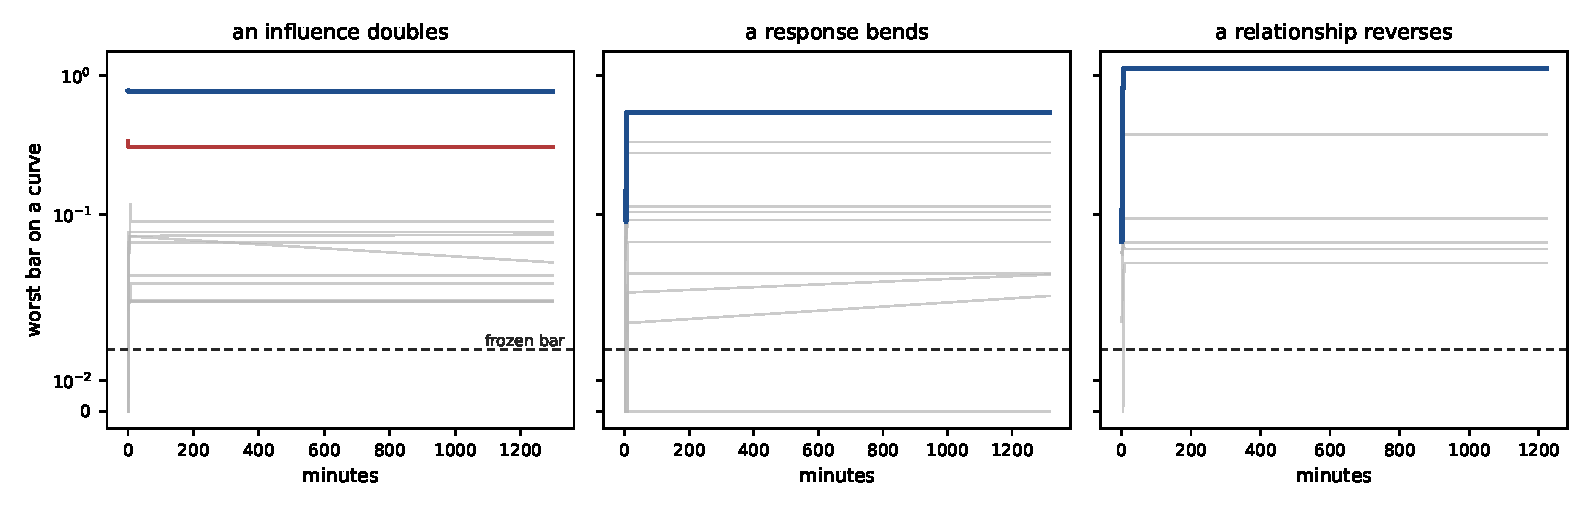
\includegraphics[width=\linewidth]{figures/fourkinds}
\caption{The three measured change kinds: each curve's worst bar
through its run (log scale; dashed line: the fixed bar). Blue: the
changed relationship. Red: the stirred neighbor, in the climb run.
Gray: every other curve. Reading line: the climb and the flip break
one relationship broadly; the bend breaks it narrowly, at the exact
knee, and the flag stands to the close.}
\label{fig:kinds}
\end{figure}

\section{Healing: what repair costs}
\label{sec:healing}

The repair mechanism --- break, notice, re-open, re-land --- is the
predecessor's published result, cited here in one sentence and never
re-litigated~\cite{p4}. What this campaign adds is the \emph{price
of repair, per kind of change, in the members' own trials}.

The slide run's close carries the signature: the six workers
finished their walks within a narrow band of trials ---
$\sim$410--415 apiece --- while the drifted node's tender closed at
$\sim$610: about two hundred extra trials, roughly half again the
walk, spent on the re-walk. One upstream neighbor closed at $\sim$700
--- re-pricing under coupling, because the drifted node sits inside
its curves: when a relationship changes, the change is paid for twice,
once at the node and once in whoever maps through it.

The climb run shows healing finishing inside the window: the
epicenter group carried the break as uncertainty through the story,
then re-walked to retirement --- converged, done --- with the
surviving curves at or below $0.089$ at the close. The flip run
shows the holding state: bars past $1.1$ at the epicenter,
\emph{pending} re-measurement --- the honest intermediate between
detection and repair, where the model knows exactly which
relationship it no longer trusts. And the bend run shows the honest
failure mode: its knee-flag stood to the close because its re-walker
was starved --- repair noticed, aimed, and never funded; the load
walls of \S\ref{sec:endure} are where that starvation lives.

The shape the three receipts share: healing is \emph{local} and
\emph{aimed}. The decay of \S\ref{sec:decay} concentrated where the
world moved; the re-walk went where the bars broke. Nobody re-learns
the whole substrate because one relationship doubled --- the model's
own error is the compass, and the price of the repair is fenced by
the same fence as the break.

\section{Endure: load and the walls}
\label{sec:endure}

Keeping a model true over a long horizon was priced by the
predecessor in a four-hour envelope: between what luck alone keeps
and what perfect hindsight would have kept, the keeper held most of
it on continuous compensation alone, without a single discrete
watering~\cite{p4}. That envelope is cited, not re-flown.

What this campaign adds is the behavior under \emph{load}, measured
on the reference grid across group sizes --- and the load walls are
named as walls, not apologized for. The \emph{turn wall}: the
turn-taking that walks the substrate degrades with
group size --- group trials per minute fell from $\sim$413 at the
reference size to $\sim$47 at the largest flown, as shared airtime
thins. The \emph{peer-motion wall}: at fixed size, when the peers are
themselves in motion, walking cadence fell from $\sim$69 to $\sim$13
--- a $5.3\times$ slowdown at a standing start. Both walls are
boundary material: the life stages of this paper are measured on the
quiet side of them, and the crossing of them is the scaling
direction the boundaries name.

\section{Carry: one regime replaced by another}
\label{sec:carry}

The transfer experiment is the lineage's first live crossing: a model
built under one regime, serving under another. The world changed
wholesale --- all six nodes at once, weights $1.0 \to 1.5$ and
response shapes linear $\to$ saturating, over a declared travel ---
and the run served through it with the same protocol throughout.
Whatever the crossing produced --- graceful service, honest
degradation, or honest refusal --- was to be the receipt.
Table~\ref{tab:transfer} is what it produced.

\begin{table}[!ht]
\centering
\small
\begin{tabular}{@{}p{0.36\linewidth}p{0.52\linewidth}@{}}
\toprule
\textbf{World} & \textbf{The model's survey} \\
\midrule
quiet (regime A) & one measuring member, six curves --- the one sender's whole
influence map \\
after the whole regime shifted (all six nodes) & two measuring members in the
change minute, twelve curves; the longest-turn member ran
$\sim$3$\times$ its siblings' trials \\
\bottomrule
\end{tabular}
\caption{Transfer: one regime replaced by another, and the survey's
answer. Reading line: localized change keeps the survey localized; a
regime change widens it --- the response fits the blast radius, same
protocol throughout.}
\label{tab:transfer}
\end{table}

\begin{figure}[!ht]
\centering
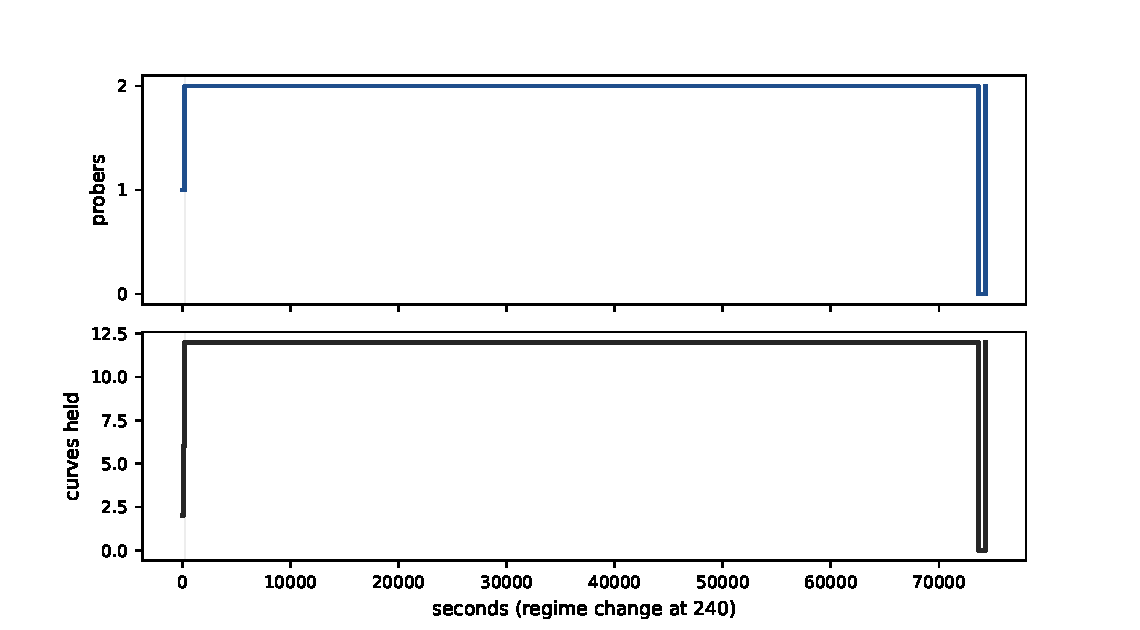
\includegraphics[width=0.8\linewidth]{figures/transfer}
\caption{Transfer, from the run's own captures: measuring members above, curves
held below; the shaded band is the declared travel of the regime
change. Reading line: one measuring member while quiet; a second joins in the
change minute and the survey doubles --- the widening fits the blast
radius.}
\label{fig:transfer}
\end{figure}

The mechanism is the same turn-taking discipline the whole lineage
runs on: one member measuring at a time per group, heartbeats,
fairness to whoever waited longest.
Under the flip of \S\ref{sec:decay} --- one member's promise broken
--- one reason meant one measuring member, and the rotation never widened.
Under the regime change, every member's world broke at once: the
turn-taking widened, a second sender joined in the change minute, and
the member that held the measuring turn longest carried roughly
three times the others' trial load. The widening is proportionate, not panicked: the model's
survey answered the blast radius of the change, and at the close the
registry purged clean. The model built under A carried into B ---
gracefully, measurably, and without anyone rebuilding it.

\section{The price: one busy evening}
\label{sec:price}

The price run is one evening, the world refusing to hold
still: a readout slide from minute five, a weight morph at minute
ten, a declared exogenous step, and --- unscheduled --- a push
through the bench's exogenous door while the morph was still
traveling. Seventeen minutes, four disturbances, one model.
Table~\ref{tab:evening} and Figure~\ref{fig:evening} hold what the
work bought; the anchors below hold what it cost.

\begin{table}[!ht]
\centering
\small
\begin{tabular}{@{}p{0.42\linewidth}p{0.24\linewidth}p{0.24\linewidth}@{}}
\toprule
\textbf{Phase of the evening} & \textbf{Mean bar} & \textbf{Worst
relationship} \\
\midrule
quiet build (first $\sim$5 min) & 0.052 & 0.073 \\
slide active ($\sim$min 5--10) & 0.054 & 0.073 \\
morph, push, and aftermath (to close) & 0.054 & 0.083 \\
\bottomrule
\end{tabular}
\caption{The busy evening, regenerated from the run's own captures
by the committed script (fixed bar 0.02). Reading line: through
three scheduled changes and one unscheduled push, the model's mean
uncertainty never left fresh-build level, and the worst single
relationship in each phase marks where each change landed and was
absorbed.}
\label{tab:evening}
\end{table}

\begin{figure}[!ht]
\centering
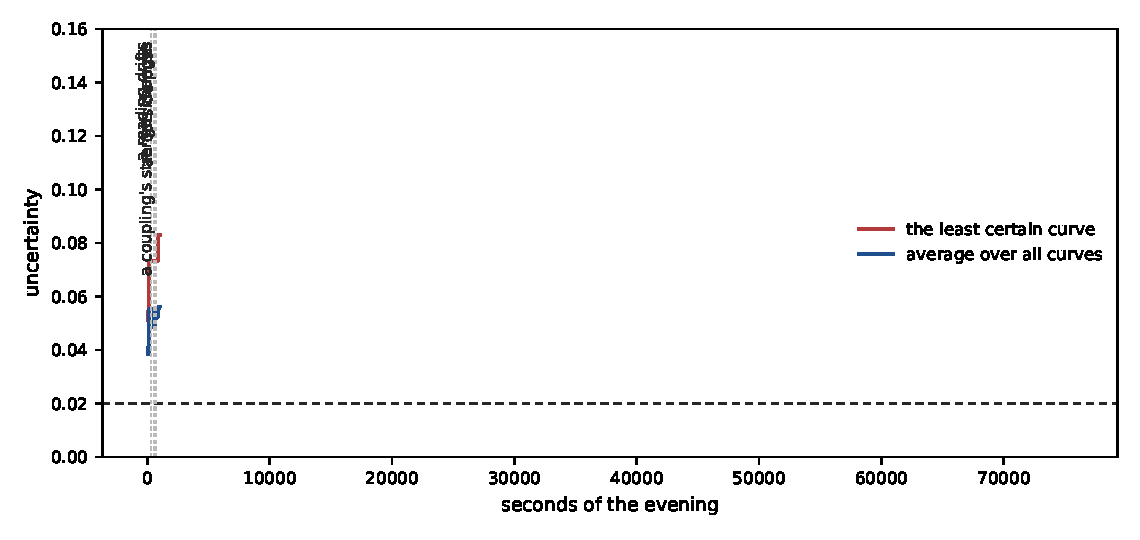
\includegraphics[width=0.85\linewidth]{figures/evening}
\caption{The busy evening, from the run's own captures. Dashed
verticals: the sensor slides, the weight morphs, the unscheduled
outside push; dashed horizontal: the fixed bar. Reading line: the
mean bar never leaves fresh-build level; the worst relationship marks
where each change landed and was absorbed back toward the bar.}
\label{fig:evening}
\end{figure}

\emph{The cost, exact.} The keeping-work totaled 13,650 trials
across the seventeen minutes --- and the load fell unevenly: two
members ran quiet (a few hundred trials apiece) while the four
re-measuring members carried 1,900--4,000 each. Keeping a model
fresh under churn costs roughly twenty times more on the members
that re-measure than on the members that stand watch. The price of
freshness is a \emph{per-member} price, not a group average --- a
budget fact for any group that would keep one model together.

\emph{The anchors.} A model left un-updated from build time --- the do-nothing
arm --- carries its build-time bars, calm-looking, while the world
moves under it: its error is invisible \emph{to itself}. The live
model paid its trials to \emph{know}: each change of the evening
surfaced as an elevated worst-relationship --- the model's own alarm
--- and was re-measured back toward the bar. The oracle arm ---
unlimited hindsight --- drives bars toward zero; the live model's
$\sim$0.05 steady state under churn \emph{is} the measured distance
from the oracle, in its own units, at this cadence and budget. The
random arm is declared as a formula from the bench's dial geometry
(analytic, analyst-side); the exact constant and the per-trial
economics --- cost per unit of recovered knowledge --- need the
per-trial ledgers and are declared owed at the evidence port,
printed here as a debt, not skipped in silence.

So the second half of the claim, in the run's own units: the
evening's knowledge was bought at a real and unevenly distributed
price, was cheaper than calm ignorance \emph{where knowing mattered}
--- the never-updated arm's calm is not knowledge --- and was honestly
measured short of hindsight, by exactly the distance the oracle
names. Cheaper where it is cheaper; honestly not where it is not.

\section{Related work}
\label{sec:related}

Each neighbor line holds one organ of this paper's subject; none
holds the assembly --- one measured causal model, born by
intervention, decaying per change kind, healing at priced cost,
transferring regimes, and kept under load, all in its own units.

\emph{Concept drift and model monitoring.} A large literature
detects that the world changed under a model --- drift detectors,
monitors, degradation dashboards. Detection is exactly one stage of
the life here, and the detector in this paper is the model's own
uncertainty structure, not an external judge.

\emph{Test-time adaptation.} Adapting a model at inference time
under distribution shift keeps predictions current; it does not
self-measure in declared uncertainty units, and it does not account
the cost of its adaptations as a priced lifecycle.

\emph{Predictive maintenance.} Schedules the upkeep of
\emph{machines} from models; here the subject is the upkeep of the
\emph{model of the substrate} itself --- the maintained thing and
the maintaining knowledge are the same object, priced in its own
trials.

\emph{Digital twins.} Live models of running systems, typically
engineering simulators built from first principles or fitted data.
The connectome is measured by intervention on the live substrate,
carries honest bars, decays, heals, and transfers; the twin
literature's drift concerns are detection-flavored, not a priced
life.

\emph{Knowledge-graph freshness.} Names the staleness of stored
facts and propagates it; the stored facts are not causal, not
intervention-measured, and their freshness is not priced in units of
re-acquisition.

\emph{Causal discovery.} Recovers structure from data --- the
predecessor of this lineage placed this line precisely: structure,
not lifecycle~\cite{p2}. The connectome's edges come from
interventions, and its subject here is what happens to the structure
after it is built.

\emph{Controllers that re-learn.} Adaptive model-predictive control
and its variants keep a model of a changing plant current and steer
to a setpoint~\cite{tanaskovic2017,knaup2024}; they lack the
uncertainty-unit accounting, the refusal, and the priced lifecycle.

\emph{The cost of keeping systems alive.} Self-adaptive
software~\cite{abufouda2014,abufouda2014b} and the mapping of
agentic technical debt~\cite{tukur2026} name the accumulating costs
of keeping AI-based systems viable; none measure them against a
do-nothing floor and a hindsight ceiling, in the system's own
units.

To our knowledge, no neighbor tends one measured causal model
through a whole life in its own units; we are not aware of anyone
this close. The comparison stays contained exactly as the
predecessor contained it~\cite{p4}: neighbors are placed, not raced.

\section{Boundaries}
\label{sec:boundaries}

Printed as boundaries, not apologies:

\begin{itemize}
\item \emph{The starved heal.} The bend's knee-flag was noticed and
aimed but never healed in its run: the re-walking member was starved
of trials there. Whether a fed heal collapses the flag is the
one-run follow-up; the starvation itself is load material, and the
walls of \S\ref{sec:endure} are its measured edge.
\item \emph{Scale.} The life stages are measured at the reference
group size on a quiet bench; catastrophic-size outcomes are boundary
material. The turn wall and the peer-motion wall
(\S\ref{sec:endure}) are the measured edges of the load behavior;
crossing them is the scaling direction.
\item \emph{Composition.} Wherever composed prediction is used, it
inherits the predecessor's measured boundary --- roughly two
nonlinear hops at the fixed noise level~\cite{p3} --- stated, not
hidden.
\item \emph{Causal scope.} The connectome is causal on the three
constitutive ingredients of \S\ref{sec:orientation}: variables,
directed structure by asymmetric intervention, interventional
semantics. Not claimed: counterfactual queries (the third rung) and
identification theory. The named outlook is counterfactual
\emph{imagination} on the conditioned model --- forecast from the
map, observe, narrow the bars by what was seen, re-forecast the
alternative action; the price anchors of \S\ref{sec:price} already
compute alternative worlds after the fact, and the outlook moves
that arithmetic inside the model itself.
\item \emph{The price debts.} The per-trial economics (cost per unit
of recovered knowledge) and the random arm's exact constant are
declared owed against the per-trial ledgers; the value priced here
is in the model's own units --- detection, localization, and
recovery --- not yet trial-denominated prediction error.
\item \emph{Planted truth.} Everything in this paper is measured
where truth was known --- the bench era's honesty, and its limit.
The open era is models of substrates where no answer key exists;
nothing here claims it.
\end{itemize}

\section{Conclusion}
\label{sec:conclusion}

One model, one life, measured whole. The connectome is born at a
priced cost of walking; it decays per kind of change --- broadly in
three kinds, narrowly and precisely at the bend in the fourth --- and
its own bars carry the alarm; it heals where it broke, at a cost
fenced by the same fence as the break; it endures load with its walls
named; it carries into a new regime with its survey fitted to the
blast radius; and its knowledge carries a price --- uneven across the
group, absolutely placed between calm ignorance and unlimited
hindsight. The lineage's
implicit promise closes here: the edges were found, the curves were
priced, the composition was proved, the promises were kept --- and
now the model that did all of it has had its own life measured, in
its own units, stage by stage. What flew is the smallest set of
runs that exercises the whole life; scaling and the field crossing
are the open directions, and both stand on these receipts.

\section*{Reproducibility}

The campaign flew on a self-hosted live bench --- a parameterizable
mathematical substrate in the same bench family as the predecessor
papers, carrying an event grammar in which every change is an event
with a destination and a declared clock. Nodes expose dials and
return readings; planted couplings --- chosen shapes at chosen
strengths --- carry one node's dial changes into another node's
reading; and a closed-form truth channel records what was actually
planted at every tick. Nothing planted is visible to the members:
they learn the couplings by probing, exactly as in the prior papers;
the truth channel exists only to score. Each run's record is
retained in the evidence bundles --- the per-tick truth and curve
captures through each story, the close-out stamps, the meters ---
and every figure and table of this paper regenerates from its bundle
by committed scripts. One mechanical cut is part of the regen
contract and declared: some bundles banked captures from more than
one run's window (a capture script ran across boots); the scripts
align each capture's wall-clock stamp against its bench uptime ---
constant within one run --- and keep only the run's own window,
so no number in this paper reads another run's registry. Registry identities never print; they resolve at
the evidence port. Verdicts are recomputed from recordings, never
read from run badges; the honest-close rule (an anomaly is a
receipt, a fix, and a re-fly) was exercised three times in this
campaign, and the re-flown numbers are the printed ones. Full
independent reproduction requires this estate's stack; on a
compatible bench, the scenario declarations --- per run: the
change kind, its destination, its clock and travel, the fixed bar,
the group --- plus the bundles are everything a re-run needs.

\begin{thebibliography}{99}
\itemsep0pt

\bibitem{p1} M.~Tafelmeier.
The Impulse Protocol: Non-Destructive Coupling Discovery in
Autonomous Agents. Zenodo, 2026.
\texttt{doi:10.5281/zenodo.21962956}.

\bibitem{p2} M.~Tafelmeier.
Calibration of Automatic Characterization. Zenodo, 2026.
\texttt{doi:10.5281/zenodo.22127166}.

\bibitem{p3} M.~Tafelmeier.
From Curves to Cascades: Composed Coupling Prediction Among
Autonomous Agents. Zenodo, 2026.
\texttt{doi:10.5281/zenodo.22401439}.

\bibitem{p4} M.~Tafelmeier.
The Steerwish: Intent Kept on Live Systems. Zenodo, 2026.
\texttt{doi:10.5281/zenodo.24369169}.

\bibitem{tanaskovic2017} M.~Tanaskovic, L.~Fagiano,
V.~Gligorovski.
Adaptive Model Predictive Control for Constrained, Linear Time
Varying Systems. arXiv:1712.07548, 2017.

\bibitem{knaup2024} J.~W.~Knaup, P.~Tsiotras.
Recursively Feasible Stochastic Model Predictive Control for
Time-Varying Linear Systems Subject to Unbounded Additive
Uncertainties. arXiv:2410.11107, 2024.

\bibitem{abufouda2014} M.~Abufouda.
A Framework for Enhancing Performance and Handling Run-Time
Uncertainty in Self-Adaptive Systems. arXiv:1402.2144, 2014.

\bibitem{abufouda2014b} M.~Abufouda.
Quality-Aware Approach for Engineering Self-Adaptive Software
Systems. arXiv:1402.2611, 2014.

\bibitem{tukur2026} M.~Tukur, H.~B.~Adeyemo, T.~Chen, et al.
From AI Technical Debt to Agentic Technical Debt: A Systematic
Mapping of Root Causes and Manifestations. arXiv:2608.01001, 2026.

\end{thebibliography}

\end{document}
